%!TEX encoding = UTF-8 Unicode

%!TEX root = ../compendium.tex

\Lab{\LabWeekTWELVE}

\begin{Goals}
    \item Kunna använda matriser som en datastruktur.
    \item Kunna separera modell från vy med hjälp av \emph{Model-View} uppdelning.
    \item Känna till grundläggande cellulära automata. % \eng{cellular automata}.
    % Följande rad är kanske inte aktuell, trådar tas upp i övningarna och hör inte riktigt hemma här då det är svårt att få in på ett smakligt sätt då Scala-kompilatorn och JVMen redan lyckas optimera koden så att den blir parallell.
    \item Känna till trådar, en grundläggande metod för att köra flera metoder \emph{samtidigt}.
\end{Goals}

% TODO: Some more preparations needed
\begin{Preparations}
    \item Läs igenom laborationen.
    % TODO: The following are just "fun" preparations, which will give the student more insight into the field but aren't
    %       actually required to complete the lab. They are optionals really.
    %\item Läs om Life på Wikipedia.
    %\item Läs om Cellulära automata på Wikipedia.
\end{Preparations}

\subsection{Bakgrund}

% Hur mycket bakgrund, vilken typ av bakgrund är lämplig/intressant/relevant?
Spelet Life (även kallat \emph{Conway's Game of Life} efter skaparen och matematikern John Horton Conway) simulerar en koloni av encelliga organismer som lever, förökar sig och dör på ett bräde. Varje enskild cells överlevnad bestäms av några enkla regler som beror på dess omgivning, detta är en s.k. \emph{cellulär automata}\footnote{Detta är ett exempel på s.k. `emergence' and `self-organization'}.  Spelet går ut på att simulera flera generationer av en cellkoloni.

Spelet har inga medvetna spelare (ett så kallat `zero-player game') och slutresultatet beror fullständigt på startkonfigurationen.


%Life (även kallat \emph{Conway's Game of Life} efter skaparen och matematikern John Horton Conway)
%är en cellulär automata som med enkla regler kan ge upphov till komplexa beteenden och har blivit känt som ett exempel på `emergence' and `self-organization'.

%Spelet har noll medvetna spelare (ett så kallat `zero-player game') där slutresultatet beror fullständigt på startkonfigurationen.

% TODO: Inför bild över brädet
% TODO: Inför bild över Moore grannskapet (och kanske även von Neumann grannskapet)

\subsection{Reglerna}

Reglerna i spelet är följande:

\begin{enumerate}
    \item Spelbrädet består av en matris med $n$ rader och $m$ kolumner ($n$ och $m$ brukar ibland modelleras som $\infty$, men vi kommer begränsa oss för enkelhetens skull)
    \item Varje cell i matrisen kan vid varje tidpunkt (varje generation) ha ett av två tillstånd: levande eller död
    \item Varje cells tillstånd i nästa generation bestäms av följande regler:
        \begin{enumerate}
            \item Om cellen är levande och har två eller tre grannar så lever den vidare, annars dör den.
            \item Om cellen är död och har exakt tre grannar så föds den och dess tillstånd ändras till levande, annars fortsätter den vara död.
        \end{enumerate}
\end{enumerate}


För mer om Game of Life, se Wikipedia:

\begin{enumerate}
    \item Engelska: \url{https://en.wikipedia.org/wiki/Conway's_Game_of_Life}
    \item Svenska: \url{https://sv.wikipedia.org/wiki/Game_of_Life}
\end{enumerate}


\subsection{Obligatoriska uppgifter}
	% Förslag på hur de kan bygga upp programmet:
    % 1) skapa en main-klass som öppnar ett fönster som visar ett x gånger y stort fönster.
    % 2) [Kommer inte göras] skapa en klass Cell som har attributet levande eller död. Gör en metod där man kan ändra tillståndet på cellen.
    % 3) skapa en matris av celler som alla initieras som döda.
	% 4) koppla ihop modellen och vyn så att om man genom att klicka i vyn kan ändra cellens tillstånd. Testa att det fungerar. Gör så att vyn uppdateras efter cellerna i modellen när man klickar på "next generation".
	% 5) Studera traitet Rule i filen blahblah. Implementera reglerna (ge lite förklarande kodexempel för traitet Rule eller var det finns)
	% 6) Skriv metod(er) som räknar upp generationer.
	% 7) Testa nedanstående startfigurer (inkludera bilder på t ex en slider). Beter det sig som förväntat?

    % Gör denna tasken till en preparation?

    \Task{Skapa en modell som kan visas i vyer som implementerar \code{LifeView2D}}
    % Visa gärna hur den ska se ut.

        \Subtask{Implementera ArrayMatrix2D}

        För att skapa en matris ska vi använda oss av Scalas inbyggda datastruktur \code{Array}.
        Denna datastruktur har en användbar konstruktur \code{ofDim} som vi ska använda för att skapa
        \code{y} arrayer av storlek \code{x} i en array vilket kan ses som en matris.

        Här nedan ser vi en sådan array utskriven i den vanliga notationen JSON (JavaScript Object Notation).
        Notera att arrayerna hamnar i y-ordning medans varje plats i dem hamnar i x-ordning enligt våran tidigare
        konvention med \code{y} arrayer och \code{x} platser i varje array.

\begin{Code}
[
    [0, 0, 0],
    [0, 0, 0],
    [0, 0, 0]
]
\end{Code}
        % TODO: Eventuellt kan man även visa upp LaTeX-array med positionerna utsatta såsom: (x_i, y_j)

        % TODO: Fortsätt förklara vad som behövs implementeras i ArrayMatrix2D


        \Subtask{Testa implementationen}

        För att nu testa implementationen kan man slumpa tillstånden på brädet med hjälp av metoden randomize som finns på
        alla objekt som ärver traitet \code{Matrix2D}, därför ska vi redan ha fått den gratis och kan enkelt göra följande:

\begin{Code}
// Slumpar alla celler i matrisen matrix till antingen 0 eller 1
matrix.randomize(2)
\end{Code}

        För att nu se till att allt har blivit rätt kan vi nu visa upp matrisen i terminalen med hjälp av \code{LifeConsoleView}.

\begin{Code}
// Skriver ut brädet i konsolen
LifeConsoleView.display(matrix)
\end{Code}

        Men detta testar inte för alla möjliga fel, så för säkerhets skull kan vi även testa att placera ut en s.k.\ glider i brädet med hjälp av en metod `place' som vi också får gratis på våran matris genom att ärva traitet \code{Matrix2D}.

\begin{Code}
// Placerar ut en glider med sitt övre vänstra hörn
// i positionen (3, 1), dvs på rad 2 och kolumn 4 (då vi noll-indexerar)
matrix.place(entities.glider, 4, 2)
\end{Code}

        Testa nu att rita ut brädet igen (utan randomize denna gången) för att se till att glidern hamnade rätt både med avseende på orientering och position.


    \Task{Implementera Life-regeln med hjälp av traitet Rule.}
    Nu har vi vår datastruktur för brädet på plats så nu är det dags att faktiskt implementera reglerna för Life.
    För att göra detta ska vi implementera traitet \code{Rule} som är en generalisering för hur cellulära automata implementeras.

        \Subtask{Implementera apply i ett nytt objekt LifeRule som implementerar \code{Rule}}
        Här nedan finnes specifikationen för traitet Rule, den innehåller endast en metod apply vars
        uppgift är att ta ett bräde och en plats på brädet och returnera vad denna plats ska ha för
        värde i nästa generation.

\begin{ScalaSpec}{Rule}
// apply tar en matrix samt en position i matrisen (i, j)
//och applicerar regeln på den positionen
def apply(m: SizedMatrix2D, i: Int, j: Int): Cell
\end{ScalaSpec}

        När denna implementeras är det viktigt att ta hänsyn till om grannarna faktiskt finns (då vårat bräde är av begränsad storlek).
        För detta bör man använda isWithinMatrix metoden som tidigare implementerades i ArrayMatrix2D.

        \Subtask{Testa implementationen}
        % TODO: Flytta Rule.applyForEntireBoard till Matrix2D.applyRule?
        För att nu i praktiken använda våran regel kan vi använda oss av metoden applyForEntireBoard som återfinns i traitet \code{Rule}.

        Om man har problem med att sin regel inte beter sig som förväntat så man returnera antalet grannar istället
        för cellens levande/död tillstånd. Efter att applicera hela s.k.\ \code{NeighborsRule} kan man visa upp resultatet med LifeConsoleView för att se om programmet räknar sina grannar korrekt.


    \Task{Skapa en ny modell som `wrappar' i kanterna}
    Just nu har vi ett beteende i modellen så att alla celler utanför brädet i praktiken räknas som döda.
    För att få ett lite mer intressant beteende så vill vi nu göra så att om en glider åker in i höger vägg
    ska den komma ut ur vänster vägg. Vi kan utgå från våran tidigare ArrayMatrix2D genom att enkelt ärva den.

        \Subtask{Skugga \code{get} så att hämtningar utanför brädet wrappar}
        % TODO: Skriv. Förklara modulo-matten?

        \Subtask{Skugga \code{isWithinMatrix} så att alla positioner är giltiga}
        % TODO: Skriv.


Intressanta mönster:

\begin{enumerate}
    \item \url{https://en.wikipedia.org/wiki/Spacefiller}
    \item \url{https://en.wikipedia.org/wiki/Spaceship_\%28cellular_automaton\%29}
\end{enumerate}

Intressanta resurser:

\begin{enumerate}
    \item Eric Weisstein's treasure trove of The Game Of Life: \url{http://www.ericweisstein.com/encyclopedias/life/topics/}
\end{enumerate}


\subsection{Frivilliga extrauppgifter}

Inom cellulära automata finns det många intressanta fenomen och beteenden,
för den som vill utforska mer av denna lilla värld så finns det här nedan en stor mängd extrauppgifter som den
intresserade läsaren kan försöka implementera till stor glädje då resultaten kan vara djupt tillfredställande.

Dessa extrauppgifter är listade i svårighetsordning och har inga beroenden på varandra (om inte annat sägs).

% Uncertain if any of these will be upgraded to obligatory assignments

\Task{Implementera andra regler för cellulära automata.}

    Det finns massor med regler för cellulära automata med sina egna intressanta beteenden och tillstånd.
    Gör den eller de du tycker verkar mest intressant!

    Fler regler kan finnas här: \url{https://en.wikipedia.org/wiki/Category:Cellular_automaton_rules}

    Nedan följer några roliga exempel som valts ut och anses lämpliga.

    \Subtask{Implementera cyklisk cellulär automata.}

        Denna typ av automata kallar cyklisk just för att det finns $N$ möjliga tillstånd och när tillståndet N-1 nås så är `nästa' tillstånd $0$.
        Detta beteendet kan beskrivas med modulo-operatorn: $T_{nästa} = T_{nuvarande} + 1 \% N$

        Regeln för att en cell byter tillstånd ges av att om en granne till den aktuella cellen har tillståndet exakt ett över cellens tillstånd så får cellen sin grannes tillstånd.

        För att få intressant beteende brukar man initialisera hela brädet så att varje cell får ett slumpvalt tillstånd.

        \url{https://en.wikipedia.org/wiki/Cyclic_cellular_automaton}

    \Subtask{Implementera Wireworld}

        Wireworld är annorlunda från andra cellulära automata då man i Wireworld designar `kretsar' inte helt olika de som finns i moderna datorer.
        På grund av detta är majoriteten av celler vanligtvis fast i ett dött tillstånd (isolatorer).

        I Wireworld kan man skapa komponenter såsom dioder och transistorer. Med dessa bygga logiska grindar och därmed hela datorer (dock väldigt långsamma sådana).

        \url{https://en.wikipedia.org/wiki/Wireworld}

        % TODO: Eventuellt ta bort och istället referera till med en länk
        \begin{figure}[h]
            \begin{center}
                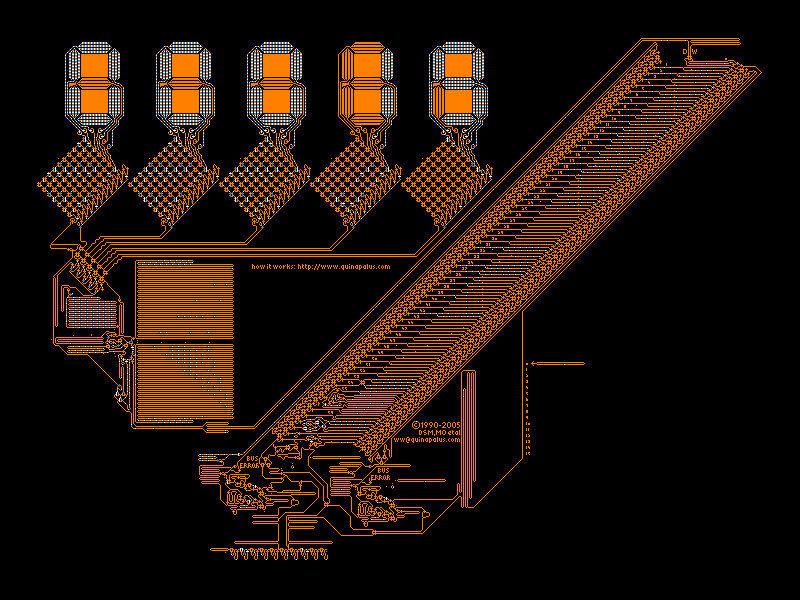
\includegraphics[width=0.8\textwidth]{../img/w12-lab/wireworld_computer.png}
            \end{center}
            \caption{En enkel dator implementerad i Wireworld}
            % Källa: Wikipedia (https://commons.wikimedia.org/wiki/File:Quad_tree_bitmap.svg)
        \end{figure}

        Ett exempel på ett projekt där en enkel dator implementerats i Wireworld finnes här: \url{http://www.quinapalus.com/wi-index.html}


\Task{Implementera spara och ladda}

    \Subtask{Spara brädets tillstånd.}
        Tillståndet ska sparas till ett format som både är lätt att spara/exportera och ladda/importera.
        Förslagsvis kan man använda formatet CSV (Comma Separated Values) eller helt enkelt bara skriva
        ut matrisen rad för rad där varje cell skrivs ut som en etta eller nolla.

    \Subtask{Ladda in det exporterade tillståndet.}
        Implementera en metod för att läsa in det sparade tillståndet


% Kanske för nästa år
%\Task{Alternativ vy: Kör programmet i webbläsaren med Scala.js}


% Detta kan kräva speciell IDE (android-studio) och eventuellt en Android-emulator som inte kan köras på skolans datorer.
%\Task{Alternativ vy: Kör programmet på Android}


% Detta kommer antagligen inte ske då det lägger till signifikant komplexitet
% En bättre extrauppgift är att representera brädet som ett quadtree då det leder en in på Hashlife
%\Task{Implementera brädet som en sparse-matris}

%I den tidigare lösningen har vi allokerat en hel matris där bara en del av brädet vanligtvis är levande, en sådan matris kallas för en sparse matris (en matris där majoriteten av värdena är 0).
%    \Subtask{???}

\Task{Implementera den supersnabba Hashlife}
    Detta är en utmaning som kräver en viss kunskap om algoritmer och hashning som läsare av denna labben inte ännu förväntas inneha.
    Den verkligt intresserade läsaren kan dock se denna uppgift som ett långtids-läromål och återkomma till uppgiften senare i sin utbildning när
    hen känner sig redo.

    En utförlig beskrivning om hashlife och quadtrees finnes på Wikipedia:
    \begin{enumerate}
        \item https://en.wikipedia.org/wiki/Hashlife
        \item https://en.wikipedia.org/wiki/Quadtree
    \end{enumerate}

    \Subtask{Implementera QuadtreeMatrix2D}
        Hashlife använder sig inte av en matris-representation för brädet utan använder sig istället av en datastruktur som heter Quadtrees.
        Dessa fungerar som vanliga träd fast varje nod kan antingen ha exakt 4 brancher eller vara ett löv. Varje branchning delar upp en kvadrat
        i 4 mindre kvadrater och varje löv representerar värdet för en kvadrat.

        Quadtrees möjliggör att man kan beräkna tomma områden på brädet på konstant tid då man vet att ett helt område kommer förbli opåverkat utan
        att behöva titta igenom varje cell.

        \begin{figure}[h]
            \begin{center}
                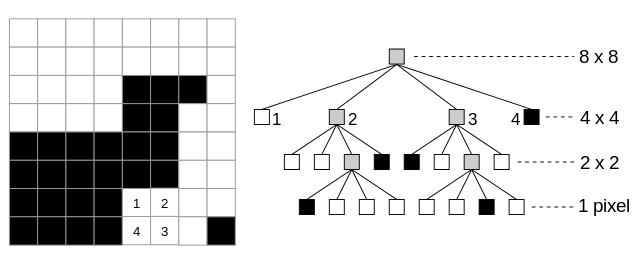
\includegraphics[width=0.7\textwidth]{../img/w12-lab/quadtree_bitmap.png}
            \end{center}
            \caption{Ett exempel på hur ett Quadtree använts för att representera en bitmap likt den som återfinns i Life}
            % Källa: Wikipedia (https://commons.wikimedia.org/wiki/File:Quad_tree_bitmap.svg)
        \end{figure}

    \Subtask{Implementera hashlife}

        Här kan vi inte handleda er, då det anses vara allt för långt utanför kursmålen. Men för den ambitiösa studenten refererar vi glatt till Wikipedia och önskar er lycka till!
